\chap{The runtime}{runtime}
\section{Notes}

There are multiple, possibly orthogonal issues.  Limit checks and garbage
collections are a little overloaded in their roles, because they also
support preemptive thread switching and interrupt handling.  Forcing
frontier to be 0 and hitting a limit check (even a zero byte limit check)
will invoke the GC, which will switch to the pending thread.

Recall that a limit check with bytes = 0 really means a check for LIMIT\_SLOP
bytes (currently LIMIT\_SLOP = 512).

\section{Bootstrap}

\figBegin
\centerline{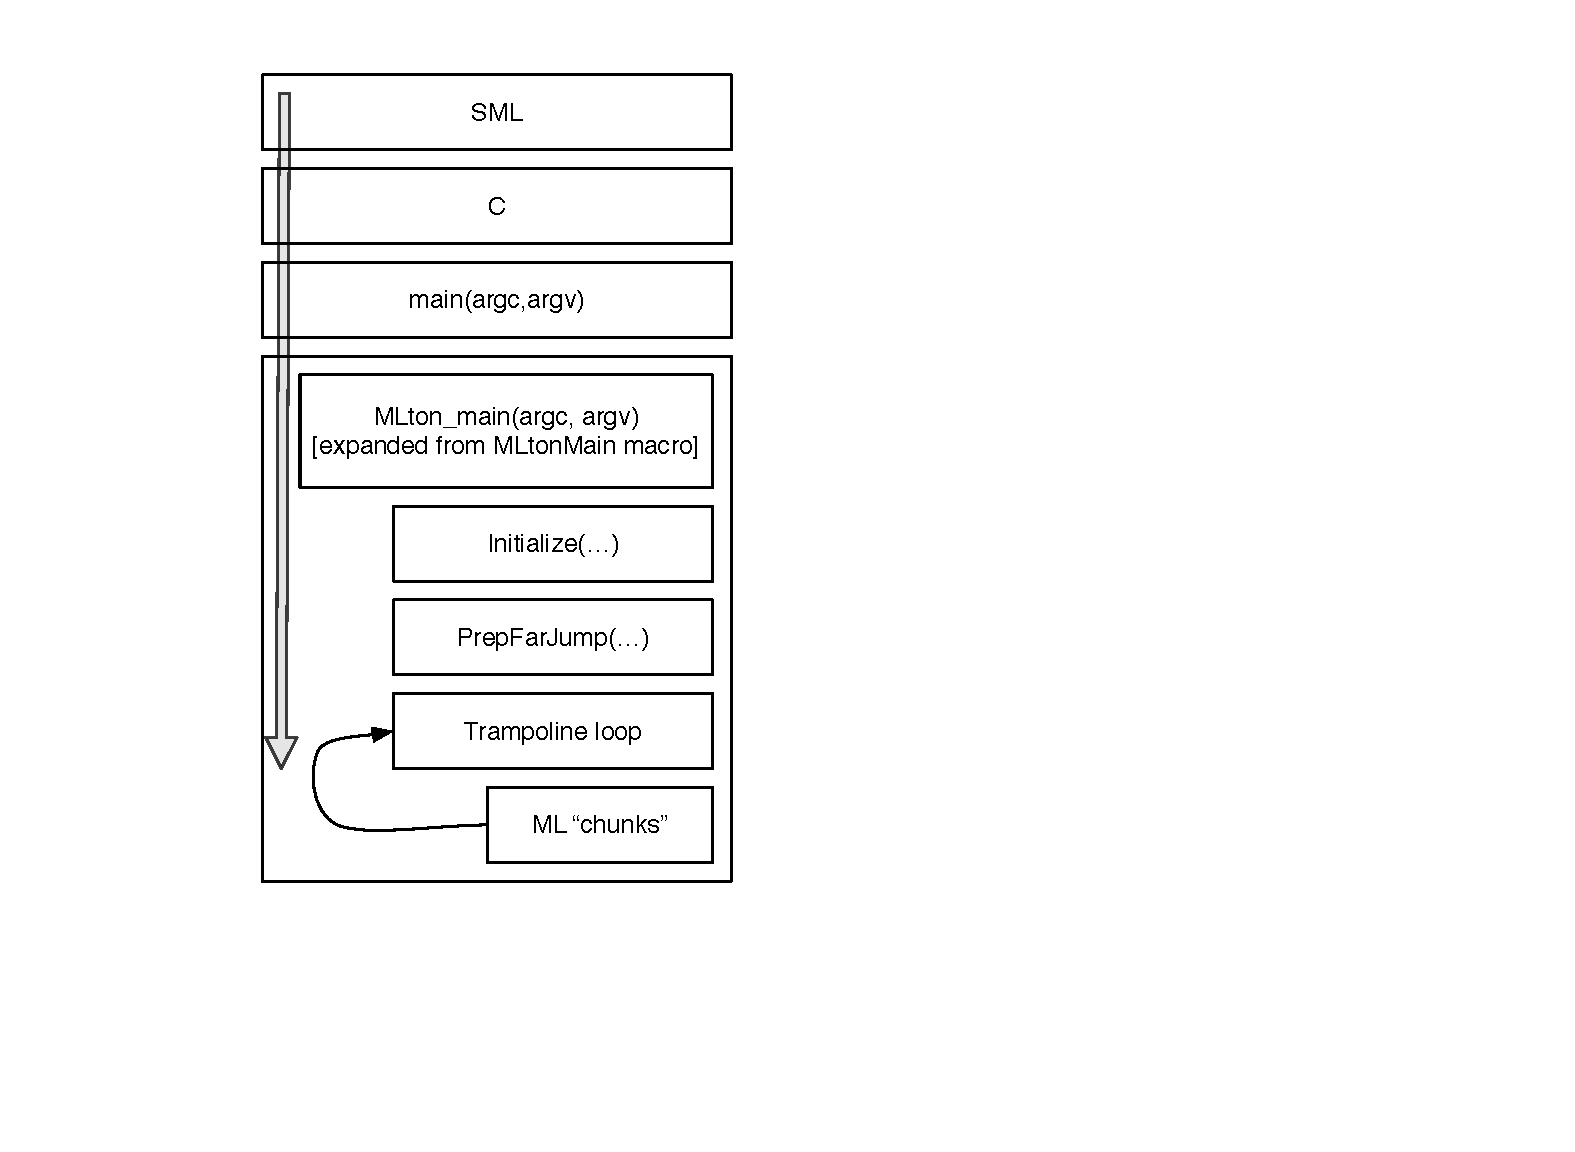
\epsfig{file=runtime-bootstrap-overview.pdf,width=2.0in}}
\figEnd{Runtime overview}{rtoverview}
       
When you compile your SML code, it is translated to machine code using one of several backends. For an in-depth description of how SML is compiled and optimized refer to~\cite{leibig:mlton-llvm-backend}. We will look at the C translation of a trivial SML program starting at the backend once all optimization phases have completed. The trivial SML program is a single statement: \texttt{val a = 2}

When reading this section of the guide, it will be useful to save the above statement as "test.sml" and then compile that using "mlton -keep g test.sml" so that you can refer to the intermediate files "test.0.c" "test.1.c" and "test.2.c"

Refer to Figure~\ref{figure:rtoverview} for an overview of how the compiler emits C code given SML code, and how control flows through the bootstrap process of the emitted code.

 
The emitted C code bootstrap at the bottom of "test.0.c" looks like this:

\begin{minipage}{\linewidth}
\lstset{language=C}\begin{lstlisting}
MLtonMain (8, 0x7CB29B69, 136, TRUE, PROFILE_NONE, FALSE, 0, 218)
int main (int argc, char* argv[]) {
    return (MLton_main (argc, argv));
}
\end{lstlisting}
\end{minipage}

\noindent and contains a \texttt{main} routine that calls \texttt{MLton\_main} which is created when the \texttt{MLtonMain} macro is expanded. 
\texttt{MLtonMain} is defined in \texttt{include/c-main.h} as a macro:

\begin{minipage}{\linewidth}
\lstset{language=C}\begin{lstlisting}
#define MLtonMain(al, mg, mfs, mmc, pk, ps, mc, ml)	
\end{lstlisting}
\end{minipage}

and ultimately calls the routine \texttt{MLton\_main (int argc, char* argv[])} 

The parameters to the \texttt{MLtonMain} macro are:

\setlist[description]{leftmargin=!,labelindent=\parindent,labelwidth=1.5cm}

\begin{description}
\item[al] alignment width (\texttt{-align})
\item[mg] a magic random number used for saving/restoring the world. This number is generated at compile time by \texttt{mlton/codegen/c-codegen/c-codegen.fun} and allows the application to save and restore its state (\htmladdnormallink{MLtonWorld}{http://mlton.org/MLtonWorld})
\item[mfs] the maximum frame size
\item[mmc] whether or not the mutator marks cards. This is an optimization strategy used by the generational GC.
\item[pk] the kind of profiling to perform (compile time option)
\item[ps] whether stack profiling is enabled (\texttt{-profile-stack})
\item[mc] the number of the first chunk to jump to
\item[ml] the function number in the chunk to jump to
\end{description}

The first six of these parameters are passed to \texttt{Initialize} (defined in \texttt{include/common-main.h}) while the final two (mc and ml) are passed to \texttt{PrepFarJump} (defined in \texttt{include/c-common.h}). 
\texttt{Initialize} sets variables in the \texttt{gcState} structure and then calls \texttt{MLton\_init(argc, argv, \&gcState)}.



\texttt{MLton\_init} (\texttt{runtime/platform.c}) initializes the posix environment, the GC and processes the runtime command line arguments.  Once \texttt{Initialize} completes, \texttt{MLton\_main} continues and calls \texttt{PrepFarJump} to prepare to jump to the first chunk of the SML program. Alternatively, it will restore the saved world and restart from where the saved program left off. Finally, \texttt{MLton\_main} goes into an infinite loop, jumping from chunk to chunk as the SML program executes.

Jumping between chunks is known as trampolining and this is done to avoid mapping highly recursive SML functions directly to C functions as this would exhaust the C stack (see \S2.2.4 of~\cite{leibig:mlton-llvm-backend}). Trampolining involves selecting a chunk from the \texttt{cont} struct and then calling to that address (pointer). You will notice that, in our example above, \texttt{mc} is set to 0 and \texttt{ml} is set to 218. That means that \texttt{PrepFarJump} will select chunk 0 to execute and will set the next function within chunk zero to 218. 

So walking through this, \texttt{PrepFarJump(0, 218)} will result in 

\begin{minipage}{\linewidth}
\lstset{language=C}\begin{lstlisting}
cont.nextChunk = (void *)Chunk0;
nextFun = 218; // note: unsynchronized global variable
\end{lstlisting}
\end{minipage}

\texttt{nextFun} is a global variable declared in \texttt{include/c-common.h}

The \texttt{Chunk0} symbol is declared in "test.0.c" via the \texttt{DeclareChunk (0)} line. This is a macro that expands to 

\begin{minipage}{\linewidth}
\lstset{language=C}\begin{lstlisting}
PRIVATE struct cont Chunk0(void);
\end{lstlisting}
\end{minipage}

The actual \texttt{Chunk0} routine is defined in "test.2.c" via the line \texttt{Chunk (0)} which is another macro (defined in \texttt{include/c-chunk.h}) that expands to:

\begin{minipage}{\linewidth}
\lstset{language=C}\begin{lstlisting}
	
        DeclareChunk(0) {
                struct cont cont;
                Pointer frontier;
                uintptr_t l_nextFun = nextFun; // remember this is 218
                Pointer stackTop;
\end{lstlisting}
\end{minipage}

Note that a local copy of the nextFun variable is made. \texttt{DeclareChunk} is, you guessed it, a macro (defined in \texttt{include/c-common.h}) and results in the above expanding to:


\begin{minipage}{\linewidth}
\lstset{language=C}\begin{lstlisting}
PRIVATE struct cont Chunk0(void) {
                struct cont cont;
                Pointer frontier;
                uintptr_t l_nextFun = nextFun; // remember this is 218
                Pointer stackTop;
\end{lstlisting}
\renewcommand{\lstlistingname}{Code}
\end{minipage}

And so we finally have our \texttt{Chunk0} routine which is what we set \texttt{chunk.nextChunk} to above if you recall.





Given the above, the trampoline section of \texttt{MLton\_main} (again, in \texttt{include/c-main.h}) will call


\begin{minipage}{\linewidth}
\lstset{language=C}\begin{lstlisting}
// equivalent in our example to cont = Chunk0();
cont=(*(struct cont(*)(void))cont.nextChunk)(); 
\end{lstlisting}
\end{minipage}

We will see, as we fully expand \texttt{Chunk0} how it ultimately returns a \texttt{cont} structure to allow us to trampoline to the next chunk. Also, we will see how each chunk routine is a large \texttt{switch} statement indexed by nextFun and so, architecturally, MLton aggregates SML functions into large C-functions where each SML function is one of the cases in the switch statement. This is how MLton minimizes the growth of the C-stack -- recursive SML functions can be aggregated into the same C function and "call" each other by manipulating \texttt{nextFun} and \texttt{switch}ing between each other. \texttt{goto} is also used to switch between SML functions without incurring any C-stack growth.

Continuing on, we are now in the \texttt{Chunk0} routine which we see, from examining "test.2.c", continues past the \texttt{Chunk (0)} line as such:

\begin{minipage}{\linewidth}
\lstset{language=C}\begin{lstlisting}
Chunk (0)
        CPointer Q_0;
        CPointer Q_1;
        CPointer Q_2;
	.
	.
	.
ChunkSwitch (0)
case 5:
L_9:
        Push (-8);
	.
	.
	.
case 218:
        G(Word32, 0) = CPointer_lt (O(CPointer, GCState, 40), StackTop);
        BNZ (G(Word32, 0), L_8);
        G(Word64, 0) = CPointer_diff (O(CPointer, GCState, 1360), Frontier);
        G(Word32, 1) = WordU64_lt (G(Word64, 0), (Word64)(0x1090ull));
        BNZ (G(Word32, 1), L_8);
        goto L_2;
L_8:
        S(CPointer, 0) = 5;
        Push (8);
        FlushFrontier();
        FlushStackTop();
        GC_collect (GCState, (Word64)(0x1090ull), (Word32)(0x0ull));
        CacheFrontier();
        CacheStackTop();
        goto L_9;
EndChunk
\end{lstlisting}
\end{minipage}

Examining this routine, let's first look at the bottom \texttt{EndChunk} which is a macro (defined in \texttt{include/c-chunk.h}) and expands to:

\begin{minipage}{\linewidth}
\lstset{language=C}\begin{lstlisting}
                default:
                        /* interchunk return */
                        nextFun = l_nextFun;
                        cont.nextChunk = (void*)nextChunks[nextFun];
                        leaveChunk:
                                FlushFrontier();
                                FlushStackTop();
                                return cont;
                    } /* end switch (l_nextFun) */
                } /* end while (1) */
        } /* end chunk */	
\end{lstlisting}
\end{minipage}

This results in \texttt{nextFun} (the global) being set to the next function in the switch statement to execute and then it sets \texttt{cont.nextChunk} to the next chunk (if we need to switch between C functions) and finally it flushes some registers and returns. Note that \texttt{nextChunks} is a list, indexed by SML function number, that lets us figure out which C-function contains the SML function we want to switch to. In our example, \texttt{nextChunks[218]} would contain a pointer to the C-function \texttt{Chunk0}. Since C-functions never call each other, but always \texttt{return} to the trampoline, the C-stack effectively does not grow while our program executes. If an SML function calls another SML function that is in the same C-function (Chunk0 in our case) we will not \texttt{return} but instead will "fall through" to the end of the \texttt{while} loop, taking us back to the top of the \texttt{switch} statement and then into the called SML function. In this way, SML functions can transition ("switch") between each other without any effect on the C-stack. Also note the label \texttt{leaveChunk} allows SML functions to jump out of the C function. The "end while (1)" refers to a while statement in the macro \texttt{ChunkSwitch} which we will now look at, before bringing this all together into a single C function.

Moving backwards, now, we look at the \texttt{CPointer} lines. These are variables that have been promoted to the top level by the AST pass of the compiler. Next we come to the \texttt{ChunkSwitch} statement. This is a macro (defined in \texttt{include/c-chunk.h}) that emits:

\begin{minipage}{\linewidth}
\lstset{language=C}\begin{lstlisting}
                CacheFrontier();
                CacheStackTop();
                while (1) {
                top:
                switch (l_nextFun) {
\end{lstlisting}
\end{minipage}

This fragment sets up the while loop that is referred to in the comment in \texttt{EndChunk} and we see the switch statement that keys on the value of \texttt{l\_nextFun} which, if you remember, is 218 in our example. Now we can look at the entire function, with most of the larger macros (but not all of them) expanded. Notice that functions can jump directly to the top of the switch statement in order to move to a different SML function without incurring any C-stack cost.

\lstset{language=C,escapechar=|}\begin{lstlisting}
PRIVATE struct cont Chunk0(void) {
    struct cont cont;
    Pointer frontier;
    uintptr_t l_nextFun = nextFun; // remember this is 218
    Pointer stackTop;
 
    CPointer Q_0;
    CPointer Q_1;
    CPointer Q_2;
	.
	.
	.
    CacheFrontier();
    CacheStackTop();
    while (1) {
       top:|\label{line:topofswitch}|
       switch (l_nextFun) {
       case 5:
       L_9:
           Push (-8);
	   .
	   .
	   .
       case 218:|\label{line:ourentryfunction}|
           G(Word32, 0) = CPointer_lt (O(CPointer, GCState, 40), StackTop);
           BNZ (G(Word32, 0), L_8);
           G(Word64, 0) = CPointer_diff (O(CPointer, GCState, 1360), Frontier);
           G(Word32, 1) = WordU64_lt (G(Word64, 0), (Word64)(0x1090ull));
           BNZ (G(Word32, 1), L_8);
           goto L_2;|\label{line:jumpwithinswitch}|
       L_8:
           S(CPointer, 0) = 5;
           Push (8);
           FlushFrontier();
           FlushStackTop();
           GC_collect (GCState, (Word64)(0x1090ull), (Word32)(0x0ull));
           CacheFrontier();
           CacheStackTop();
           goto L_9;
       default:
           /* interchunk return */
           nextFun = l_nextFun;
           cont.nextChunk = (void*)nextChunks[nextFun];
           leaveChunk:
               FlushFrontier();
               FlushStackTop();
               return cont;
        } /* end switch (l_nextFun) */
     } /* end while (1) */
} /* end chunk */	
\end{lstlisting}

Some interesting things: note line~\ref{line:ourentryfunction} which is the piece of code that \texttt{MLton\_main} ultimately executes the first time we enter the trampoline section after preparing the cont structure in \texttt{PrepFarJump}. Also, line~\ref{line:jumpwithinswitch} shows how SML functions that correspond to each case statement can jump around within the case statement itself -- control is in no way linear in the emitted C code. We omitted the code at \texttt{L\_2} for brevity, but you can look in "test.2.c" as a reference.

Also, note again line~\ref{line:topofswitch} which is the top of the switch statement. There is another macro, that isn't referenced in the example code we've shown here, that uses that label to switch back to the caller. The macro is \texttt{Return()} and it pops (but does not adjust the size of the stack) the caller off of the SML stack and then jumps to \texttt{top} in order to switch back ("return") to the calling function. The code for \texttt{Return()} follows. Note the setting of \texttt{l\_nextFun}. 

\begin{minipage}{\linewidth}
\lstset{language=C}\begin{lstlisting}
       l_nextFun = *(uintptr_t*)(StackTop - sizeof(void*));
       goto top;
\end{lstlisting}
\end{minipage}

SML functions themselves, once translated down to C, are essentially all pointer and memory manipulation. Let's look at the section of code for \texttt{case 218}.

\begin{minipage}{\linewidth}
\lstset{language=C}\begin{lstlisting}
       case 218:
           G(Word32, 0) = CPointer_lt (O(CPointer, GCState, 40), StackTop);|\label{line:gmacro1}|
           BNZ (G(Word32, 0), L_8);
           G(Word64, 0) = CPointer_diff (O(CPointer, GCState, 1360), Frontier);
           G(Word32, 1) = WordU64_lt (G(Word64, 0), (Word64)(0x1090ull));|\label{line:frontier1}|
           BNZ (G(Word32, 1), L_8);
           goto L_2;
       L_8:
           S(CPointer, 0) = 5;
           Push (8);
           FlushFrontier();
           FlushStackTop();
           GC_collect (GCState, (Word64)(0x1090ull), (Word32)(0x0ull));
           CacheFrontier();
           CacheStackTop();
           goto L_9;
\end{lstlisting}
\end{minipage}

As we pointed out, once you get into the C code, it is all pointer and memory manipulation via a handful of macros. In the above code, we have four macros and two C-functions (that are inline-able and so should not affect the C-stack). The macros are defined in \texttt{include/c-chunk.h} and do the following:

\begin{description}
\item[G] sets a global statically allocated variable for temporary use
\item[O] retrieves the value at a particular memory offset and casts it to a specified type/width
\item[BNZ] branch if not zero
\end{description}

For the \texttt{G} macro on line~\ref{line:gmacro1}, we have the following expansion:
\texttt{G(Word32, 0)} becomes \texttt{globalWord32[0]} which refers to a statically allocated array in "test.0.c" \texttt{PRIVATE Word32 globalWord32 [2]}. On the other side of the assignment we have \texttt{CPointer\_lt (O(CPointer, GCState, 40), StackTop)} which is a C-function call and a macro that expands to:

\begin{minipage}{\linewidth}
\lstset{language=C,numbers=none,frame=none}\begin{lstlisting}
    G(Word32, 0) = CPointer_lt (O(CPointer, GCState, 40), StackTop);
    // expands to:
    globalWord32[0] = CPointer_lt ((*(CPointer*)((GCState) + (40))), StackTop);
\end{lstlisting}
\end{minipage}

which is comparing the value of the field that is 40 bytes into GCState with the value of StackTop. This offset is calculated by the compiler and should correspond to the fifth field (\texttt{GCStat.exnStack}) since our alignment was 8. So we are checking if exnStack $<$ stackTop and if it is, globalWord32[0] is set to true (1). If it is true, we jump to L\_8 because a GC is needed, otherwise we check (line~\ref{line:frontier1}) to see if there's at least 0x1090 bytes of space left before we hit the Frontier, and if that's not true we again need to GC, otherwise we can proceed to label L\_2.

\section{Stacks}

MLton uses green threads. These are managed entirely in user space by your application. Only one thread runs at a time and each thread has its own stack. The global state structure (\texttt{GC\_state}) has fields that point to the stack of the currently running thread.

At startup (\texttt{init-world.c}) MLton creates a new thread and then switches to it. The act of switching copies a pointer to the thread's stacks into the \texttt{GC\_state} structure. MLton's main loop (trampoline) operates entirely out of that structure, so this effectively runs the thread.

When another new thread is created (\texttt{new-object.c}), MLton allocates a new thread object (see \texttt{thread.h}) which has pointers to the newly allocated thread stack and exception stack. The running thread can then (optionally) "switch" to that thread which, as mentioned above, copies the new threads stack pointers into \texttt{GC\_state} and then resumes the trampoline loop.

A thread stack is itself a block of heap allocate memory, the beginning of which corresponds to the \texttt{GC\_stack} struct format. This struct tracks a few items related to garbage collection and also the total and used stack size. So the stack block itself might be 100 bytes, the struct only overlays the first 20-32 bytes (depending upon architecture) with the rest of the block being ostensibly unstructured. 

However, the rest of the block is actually a sequence of stack frames. These frames are pushed onto the stack as needed based on what function is being called. When they are pushed, the stacktop is extended by a size corresponding to the frame being pushed. When the function returns, the stacktop is moved back down by the appropriate size, thereby reclaiming space on the stack for future function calls. 

Since the compiler is able to derive what data will be stored in each frame, a frame will have a predetermined size and format. The start of each frame consists of a label indicating the type of frame, a pointer to an array of frame offsets, and the size of the frame. The offsets (relative to the base of the frame) are used to determine where in the frame each object pointer lives. 

Since you can not determine exactly how many function calls may occur (or in what order) at compile time, the stack grows when necessary. This is handled by the garbage collector by making a copy of the current stack into a new, larger, memory area, and then updating the stack pointers in the thread structure. 

